% !TEX root = ../sparsity_thesis.tex
\chapter{Literature Review}
\label{ch:literature-review}

This chapter surveys the state of the art at the intersection of Explainable
Artificial Intelligence (XAI), enterprise machine learning, multi-tenant
Software-as-a-Service (SaaS) architectures, and the cold-start problem. The
chapter is organized into three sections: a review of representative previous
research with explicit identification of its limitations
(Section~\ref{sec:lit-prev}), a theoretical review of the concepts and
mathematical foundations on which this thesis rests (Section~\ref{sec:lit-theory}),
and the research thinking framework that links these components into a single
causal chain (Section~\ref{sec:lit-framework}).

\section{Review of Previous Research}
\label{sec:lit-prev}

Each study is assessed not only for its individual contribution but, more
importantly, for the degree to which it leaves the specific research gap
addressed by the present thesis unresolved.

\begin{table}[h]
\centering
\caption{Literature review of previous research.}
\label{tab:literature-review}
\renewcommand{\arraystretch}{1.25}
\begin{tabularx}{\textwidth}{@{}p{3.4cm} p{2.7cm} X@{}}
\toprule
\textbf{Title} & \textbf{Researcher} & \textbf{Explanation} \\
\midrule
A Unified Approach to Interpreting Model Predictions
& Lundberg \& Lee (2017)
& Introduced SHAP (SHapley Additive exPlanations), unifying six prior
attribution methods under a single game-theoretic framework grounded in Shapley
values from cooperative game theory. Demonstrated empirically that SHAP
attributions are locally accurate and globally consistent on standard benchmark
datasets (UCI Adult, MNIST). The study, however, evaluates SHAP exclusively on
data-rich datasets and offers no analysis of how attribution fidelity behaves
when the underlying model is trained on extremely small samples; consequently
it does not address the degradation of explanation reliability under
tenant-level data sparsity, which is the central concern of the present work. \\

``Why Should I Trust You?'': Explaining the Predictions of Any Classifier
& Ribeiro, Singh \& Guestrin (2016)
& Proposed LIME (Local Interpretable Model-agnostic Explanations), which fits a
sparse linear surrogate to a perturbation neighbourhood of each instance to
recover locally faithful feature attributions for any black-box classifier.
Validated on text and image classifiers and credited with seeding the modern
XAI field. The study assumes that the underlying classifier itself is
competent; it neither defines nor measures the failure mode in which LIME
continues to emit confident explanations on top of a model that has collapsed
to random performance---the \emph{hallucinated explanation} phenomenon central
to this thesis. \\

Fooling LIME and SHAP: Adversarial Attacks on Post-hoc Explanation Methods
& Slack \emph{et al.}\ (2020)
& Demonstrated that adversarially-constructed classifiers can deliberately
deceive both SHAP and LIME, producing innocuous-looking attributions that mask
discriminatory behaviour. This was a foundational result on the \emph{fragility}
of post-hoc explanations. However, the failure mode considered is adversarial
and intentional; the study does not investigate the non-adversarial,
structurally-induced failure of these explainers when training data is
naturally scarce, as occurs by design in cold-start multi-tenant SaaS
environments. \\

Multi-Tenant SaaS Applications: Maintenance Dream or Nightmare?
& Bezemer \& Zaidman (2010)
& Provided one of the most-cited characterizations of the multi-tenant SaaS
architecture, including the trade-offs between shared-schema, schema-per-tenant
and database-per-tenant isolation models from a software-maintenance
perspective. The work focuses on operational, security and maintainability
concerns of multi-tenancy; it does not consider the downstream consequence of
tenant-level data silos for embedded ML and XAI subsystems, and therefore does
not anticipate the explanatory cold-start regime that this thesis identifies. \\

Addressing Cold Start in Recommender Systems: A Semi-Supervised Co-Training
Algorithm
& Zhang, Cao \& Yeung (2014)
& Surveyed and proposed a hybrid semi-supervised approach to mitigate the
cold-start problem in collaborative-filtering recommender systems, where new
users or items lack interaction history. Defined the cold-start problem in
strictly \emph{predictive} terms: insufficient data to generate an accurate
recommendation. The study, like the wider cold-start literature, does not
distinguish between predictive cold-start and \emph{explanatory} cold-start,
and offers no mechanism by which a system might preserve user trust through
architectural routing when explanations---rather than predictions---become
unreliable. \\
\bottomrule
\end{tabularx}
\end{table}

\paragraph{Synthesis of the Research Gap.}
Taken together, the surveyed literature establishes the methodological
foundations of SHAP and LIME~\citep{lundberg2017unified, ribeiro2016why},
exposes their adversarial fragility \citep[Slack \emph{et al.},][]{rudin2019stop},
characterizes the structural properties of multi-tenant SaaS
\citep{bezemer2010multi}, and formalizes the predictive cold-start problem in
recommender systems. Yet no identified study (i) quantifies the \emph{natural},
non-adversarial degradation of XAI fidelity as a function of tenant-level
training-data volume in a multi-tenant ERP context, (ii) operationally
distinguishes \emph{predictive} cold-start from \emph{explanatory} cold-start,
nor (iii) proposes an architectural routing gate that conditions the choice of
explanation strategy on per-tenant data maturity. This three-fold gap defines
the contribution space of the present thesis.

\section{Theoretical Review}
\label{sec:lit-theory}

\subsection{Explainable Artificial Intelligence (XAI) in Enterprise Systems}
\label{subsec:xai-enterprise}

Explainable Artificial Intelligence (XAI) denotes the family of techniques,
models, and architectural practices whose objective is to render the
predictions of machine-learning systems intelligible to human stakeholders. In
enterprise contexts, the demand for XAI is driven less by intellectual
curiosity than by operational and regulatory necessity. ML-driven decisions in
credit scoring, lead qualification, employee-attrition prediction and supplier
risk assessment carry direct economic and legal consequences; under regulatory
regimes such as the European Union's General Data Protection Regulation (GDPR,
Art.~22) and the forthcoming EU Artificial Intelligence Act, affected
individuals possess a qualified right to a meaningful explanation of automated
decisions made about them~\citep{eu2024aiact}.

The XAI literature broadly distinguishes two paradigms. The first is the
construction of \emph{intrinsically interpretable} models---decision lists,
generalized additive models, and sparse linear models---whose decision logic is
directly readable from the model itself~\citep{rudin2019stop}. The second, and
by a wide margin the more commercially deployed, is the use of \emph{post-hoc}
explainers that operate on top of a pre-trained black-box model, generating an
interpretation after the fact. \citet{rudin2019stop} argues forcefully against
the latter paradigm in high-stakes domains, on the grounds that a post-hoc
explanation is not a description of \emph{what the model does}, but rather an
approximation of what the model does that is itself subject to error. The
present thesis builds directly on this critique by demonstrating empirically
that, under data sparsity, the approximation error of post-hoc explainers
becomes large enough to invert the sign of the explanation's epistemic value:
the explanation no longer reduces uncertainty about the model's behaviour, it
manufactures false certainty.

A second methodologically important distinction is between \emph{global} and
\emph{local} explanations. Global explanations characterize the average
behaviour of the model across an entire dataset (for example, a global
feature-importance bar chart). Local explanations characterize the behaviour
of the model for a \emph{single specific instance} (``for this particular
invoice, the predicted late-payment probability is driven primarily by feature
$X$''). The shift in the XAI literature over the past decade has been
decisively towards local explanations~\citep{lipton2018mythos}, because
operational ERP decisions are made one transaction, one customer, and one
employee at a time. It is precisely the local-explanation regime---SHAP local
attributions and LIME local surrogates---that the present thesis identifies as
most vulnerable to the cold-start failure mode.

\subsection{Post-Hoc Explanation Methods: SHAP and LIME}
\label{subsec:shap-lime}

\paragraph{SHAP (SHapley Additive exPlanations).}
Mathematically, SHAP grounds the problem of feature attribution in cooperative
game theory. Consider a model $f$ and a prediction $f(x)$ for a single instance
$x$ with $M$ input features. The Shapley value $\varphi_i$ assigned to feature
$i$ is defined as the average marginal contribution of that feature across all
possible orderings in which features may be added to a
coalition~\citep{lundberg2017unified}:
\begin{equation}
\varphi_i \;=\; \sum_{S \subseteq F \setminus \{i\}}
\frac{|S|!\,(M - |S| - 1)!}{M!}
\Bigl[\,f_{S \cup \{i\}}(x_{S \cup \{i\}}) \;-\; f_S(x_S)\,\Bigr],
\label{eq:shap}
\end{equation}
where $F$ is the full set of features, $S$ is any subset of features not
containing $i$, and $f_S(x_S)$ denotes the expected model output when only the
features in $S$ are known. SHAP attributions satisfy three axiomatic guarantees
inherited from cooperative game theory---\emph{local accuracy},
\emph{missingness} and \emph{consistency}---which together motivate its
theoretical preference over earlier ad-hoc attribution methods.

Because the exhaustive Shapley summation in Equation~\eqref{eq:shap} is
exponential in the number of features, practical SHAP implementations rely on
model-class-specific approximations. The most relevant to this thesis is
\textbf{TreeExplainer}, a polynomial-time exact algorithm for tree ensembles
such as gradient-boosted decision trees and random
forests~\citep{lundberg2020local}. SHAP attributions support both local
interpretability (instance-level waterfall and force plots) and global
interpretability (aggregations such as the beeswarm summary plot and
mean-absolute-value bar charts).

\paragraph{LIME (Local Interpretable Model-agnostic Explanations).}
LIME approaches the same problem from a fundamentally different direction.
Rather than computing a closed-form attribution from the structure of the
model itself, LIME treats $f$ as an opaque oracle and fits an
\emph{interpretable surrogate} $g$ (typically a sparse linear model) to a
\emph{perturbation neighbourhood} of the instance $x$ being explained.
Formally, LIME solves~\citep{ribeiro2016why}:
\begin{equation}
\xi(x) \;=\; \underset{g \in G}{\arg\min}\;
\mathcal{L}\bigl(f,\,g,\,\pi_x\bigr) \;+\; \Omega(g),
\label{eq:lime}
\end{equation}
where $G$ is the class of interpretable surrogate models (typically sparse
linear functions), $\pi_x$ is a proximity kernel that weights perturbed samples
by their similarity to $x$, $\mathcal{L}$ is a locality-aware loss measuring
how faithfully $g$ approximates $f$ within $\pi_x$, and $\Omega(g)$ is a
complexity penalty (for example, the number of non-zero coefficients) that
enforces interpretability.

The critical theoretical observation, and the one that motivates the empirical
investigation of this thesis, is that \emph{both} SHAP and LIME are explainers
of $f$, not of the \emph{ground truth} the modeller hoped $f$ would learn. If
$f$ has been trained on a sample too small to recover the underlying
signal---as is the structural condition of cold-start tenants---then SHAP will
faithfully attribute $f$'s noisy decisions, and LIME will fit a faithful linear
surrogate to that same noise. Faithfulness to a degenerate model is not a
virtue; it is the technical mechanism by which the hallucinated explanation is
produced.

\begin{figure}[h]
    \centering
    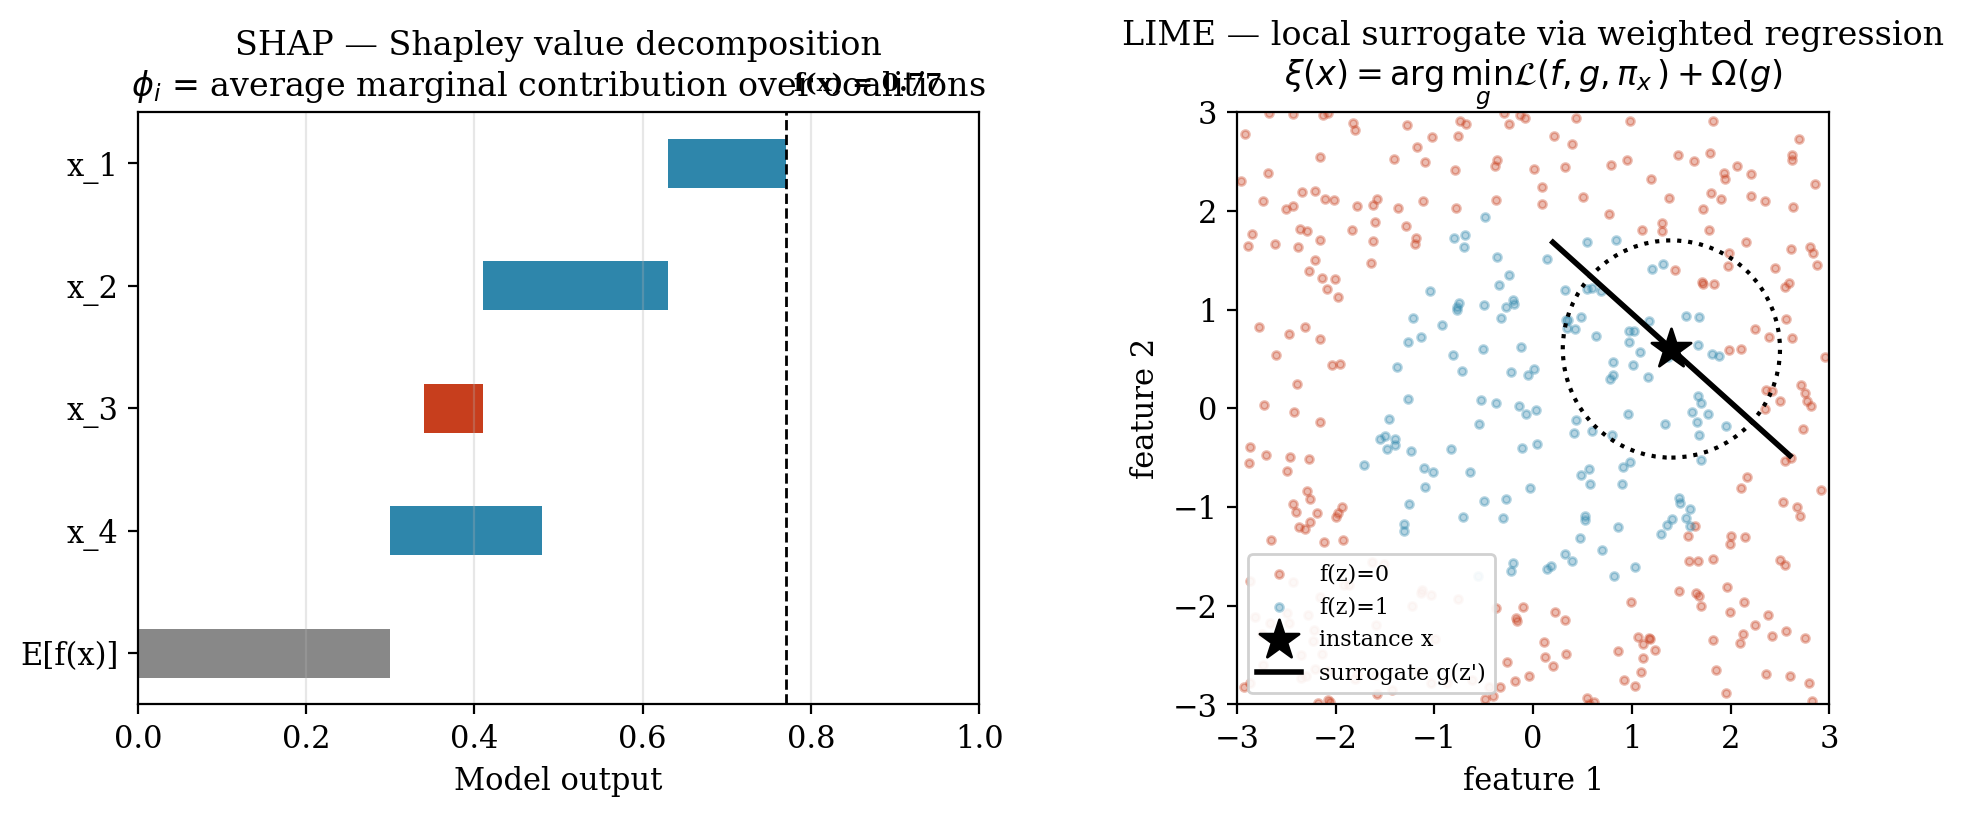
\includegraphics[width=0.95\textwidth]{sparsity_fig_2_1_shap_vs_lime.png}
    \caption{Mechanistic comparison of SHAP and LIME. SHAP (left) decomposes the
    model output $f(x)$ as the sum of the expected output $E[f(x)]$ and the
    per-feature Shapley contributions $\phi_i$; LIME (right) fits a locally
    weighted linear surrogate $g$ to perturbed samples drawn around the instance
    $x$ within the locality kernel $\pi_x$.}
    \label{fig:shap_vs_lime}
\end{figure}

\subsection{Multi-Tenant Architecture and Data Isolation}
\label{subsec:multi-tenant}

A \emph{multi-tenant} application is one in which a single deployment of the
software serves multiple independent customer organizations, called
\emph{tenants}, while preserving the logical isolation of each tenant's data,
configuration and access permissions~\citep{bezemer2010multi}. The literature
recognizes three canonical isolation models, in order of increasing isolation
strength: (i) \emph{shared schema} with a discriminator column,
(ii) \emph{schema-per-tenant} within a single database, and
(iii) \emph{database-per-tenant}, in which each tenant is allocated a
physically distinct database~\citep{krebs2014multitenancy}.

The system studied in this thesis adopts the database-per-tenant model on
PostgreSQL, orchestrated by Django~4.2 via a routed connection layer that
resolves each inbound request to the appropriate tenant database. This choice
maximizes data-isolation guarantees: a SQL injection or query-construction
error in one tenant's context cannot, by construction, leak rows belonging to
another tenant. From a security and compliance perspective the model is
conservative and defensible.

From a machine-learning perspective, however, the same isolation property has
a corrosive side effect. Each tenant's ML pipeline is confined to that
tenant's own database, which means that the training corpus available to any
per-tenant model is bounded above by the operational history of a single SME.
A tenant who joined the platform three weeks ago and has issued forty invoices
simply has no way to participate in a training process that requires thousands
of labelled observations. The isolation that protects the SME tenant's data
from its competitors also \emph{starves} the ML and XAI subsystems that the
platform offers to that same SME. This structural tension between
data-isolation security and data-volume sufficiency is the architectural
origin of the cold-start regime addressed by this thesis.

\subsection{The Cold-Start Problem in ML versus XAI}
\label{subsec:cold-start}

The traditional cold-start problem, as formulated in the recommender-systems
and personalization literature, is \emph{predictive}: a newly-introduced user
or item lacks the interaction history required for an accurate prediction to
be made. The remedies developed in that literature---content-based fallbacks,
transfer learning, meta-learning and warm-start priors---are correspondingly
aimed at improving the \emph{prediction}.

The present thesis introduces a conceptually distinct second variant, the
\emph{explanatory} cold-start. An explanatory cold-start occurs when the
system possesses enough engineering machinery to \emph{emit} a prediction and
an accompanying SHAP or LIME explanation, but the underlying model is too
poorly fit to make either the prediction \emph{or} the explanation faithful
representations of any real-world phenomenon. Critically, the failure modes of
predictive and explanatory cold-start are not aligned: a predictive cold-start
fails \emph{loudly} (the prediction is wrong and is sometimes recognized as
such), whereas an explanatory cold-start fails \emph{silently and confidently}
(a polished, axiomatically-grounded SHAP attribution is rendered for a model
that has collapsed to chance performance).

This silent failure mode is what this thesis names the \textbf{hallucinated
explanation}: an explanation that is \emph{internally} faithful (to the
degenerate model that produced it) and \emph{externally} meaningless (with
respect to the business process the model was intended to capture). The
phenomenon is not a flaw of SHAP or LIME \emph{per se}---both methods are
operating exactly as specified---but rather a failure of the surrounding
system to recognize that \emph{explaining a noise-fitting model is a category
error}. The architectural implication is that no defensible XAI deployment in
a multi-tenant SaaS context can treat the explanation layer as unconditional;
it must be guarded by a mechanism that detects the explanatory cold-start
regime and refuses to enter it.

\subsection{Metrics for Explanation Reliability}
\label{subsec:metrics}

To convert the abstract notion of ``explanation reliability'' into a
measurable quantity, this thesis adopts and combines several established
metrics from the XAI-stability literature.

\paragraph{Spearman Rank Correlation ($\rho$).}
Given two rankings of $n$ features---one produced by the explainer under
evaluation and one produced by a reference \emph{data-rich baseline} explainer
trained on the largest available data partition---the Spearman rank
correlation is defined as
\begin{equation}
\rho \;=\; 1 \;-\; \frac{6 \sum_{i=1}^{n} d_i^{\,2}}{n\,(n^2 - 1)},
\label{eq:spearman}
\end{equation}
where $d_i$ is the difference between the ranks of feature $i$ under the two
rankings. A value of $\rho = 1$ denotes perfect rank agreement (the
sparse-tenant model orders feature importances identically to the data-rich
baseline); a value of $\rho \le 0$ denotes that the two rankings are
uncorrelated or reversed. A conventional threshold of $\rho \ge 0.70$ is used
in the explanation-stability literature as the lower bound of operationally
defensible ranking agreement; below this value, the explainer can no longer
be regarded as recovering the same feature-importance signal as a
well-trained reference.

\paragraph{SHAP Absolute Variance.}
Defined as the variance of the per-feature mean absolute SHAP value across the
feature set, this metric quantifies \emph{how concentrated} the explanation
mass is on a small number of features versus how \emph{evenly distributed} it
is across many. A high SHAP absolute variance indicates that a single feature
is dominating the attribution---a signature symptom of over-fitting to a
spurious correlation in a small sample. A low variance indicates that
explanatory weight is distributed across a plausible coalition of features,
consistent with a well-regularized model. In the experimental results of this
thesis, SHAP absolute variance rises from $0.0224$ at the data-rich tier
($n = 50{,}000$) to $0.2017$ at the $n = 200$ tier, a nearly nine-fold spike
that empirically witnesses the over-fitting collapse of the sparse-tenant
model.

Complementary metrics employed in the empirical study include SHAP entropy
(an information-theoretic measure of the diffuseness of the attribution
distribution), the top-$k$ Jaccard similarity of LIME feature selections
across repeated runs (a measure of explanation \emph{stability}), and
standard predictive metrics such as AUC-ROC. The full operational definitions
are deferred to Chapter~\ref{ch:methodology}; what matters for the theoretical
framework is that, taken together, these metrics make it possible to
\emph{measure}, rather than merely assert, the degradation of explanation
reliability as a continuous function of tenant data volume.

\begin{figure}[h]
    \centering
    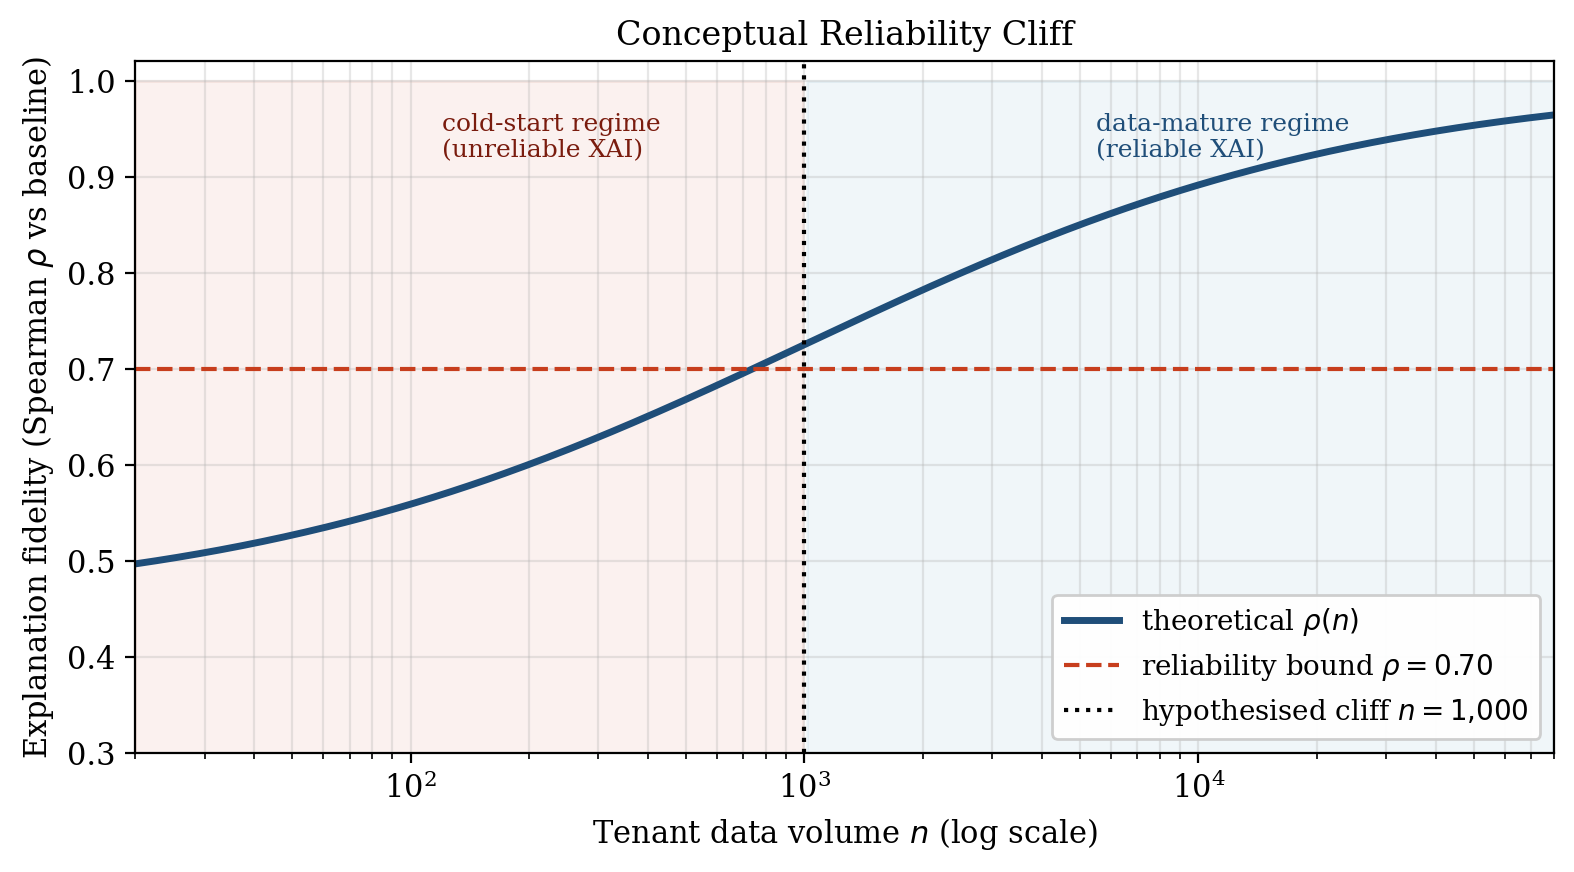
\includegraphics[width=0.85\textwidth]{sparsity_fig_2_2_reliability_cliff_theory.png}
    \caption{Conceptual \emph{Reliability Cliff} relating tenant data volume
    $n$ (log scale) to explanation fidelity (Spearman $\rho$ against the
    data-rich baseline). The horizontal dashed line marks the $\rho = 0.70$
    reliability bound; the vertical dotted line marks the hypothesised
    cold-start threshold at $n = 1{,}000$.}
    \label{fig:reliability_cliff_theory}
\end{figure}

\section{Research Thinking Framework}
\label{sec:lit-framework}

The conceptual architecture of this research connects the theoretical
components reviewed above into a single causal chain, which simultaneously
functions as the logical scaffold of the empirical study and as the blueprint
for the proposed architectural solution.

The chain begins with \textbf{multi-tenant data isolation}. The
database-per-tenant architecture adopted by the studied ERP enforces strict
logical and physical separation between tenant datasets. This isolation is
non-negotiable from a security and regulatory standpoint, yet it has the
unavoidable consequence that the data available to each tenant's ML pipeline
is bounded by that tenant's own operational history. For mature tenants this
bound is large; for cold-start SMEs it is small, sometimes vanishingly so.

This produces the second link in the chain: \textbf{data sparsity} at the
tenant level. Sparsity is not a transient anomaly but a \emph{structural}
property of the multi-tenant SaaS distribution, in which a long tail of small
tenants persists indefinitely alongside a smaller head of data-rich
enterprises.

Sparsity then propagates into the ML layer, where per-tenant models trained
on small samples regress toward random performance. Under classical ML
evaluation this is recognized as the predictive cold-start. However, in any
deployment in which SHAP or LIME is applied unconditionally to such a
degraded model, the sparsity propagates one layer further into the XAI
subsystem, producing the third link in the chain: \textbf{XAI degradation in
the form of hallucinated explanations}---confident, well-formatted
attributions over a model that has no genuine signal to attribute.

The fourth link is \textbf{empirical measurement}. Hallucinated explanations
are dangerous precisely because they do not announce themselves. The
framework therefore prescribes that the phenomenon be made visible through
quantitative metrics: Spearman rank correlation against a data-rich baseline
(fidelity), absolute SHAP variance and SHAP entropy (stability), and LIME
top-$k$ Jaccard similarity (overlap). The empirical layer of the framework
operationalizes the conceptual claim that the failure of XAI under sparsity
is not merely \emph{theoretically plausible} but \emph{empirically
measurable} and, therefore, \emph{engineering-actionable}.

The chain closes with the fifth link: \textbf{the architectural solution}.
Because the failure regime can be detected ahead of time from a single
observable property of the tenant---its row count---the framework proposes
the \textbf{Maturity-Aware AI Routing} pattern. Tenants whose data volume
falls below the empirically-identified cold-start threshold ($n \le 1{,}000$,
as established in Chapter~\ref{ch:results}) are routed to a global,
heuristic-based explanation strategy derived from the data-rich baseline;
tenants at or above the threshold receive local SHAP/LIME explanations. The
routing decision is made at the architectural layer, before any explanation
is generated, and is therefore guaranteed to prevent the rendering of a
hallucinated explanation regardless of downstream UI behaviour.

\begin{figure}[h]
    \centering
    \begin{tikzpicture}[
        node distance=6mm and 8mm,
        every node/.style={font=\footnotesize},
        box/.style={draw,rounded corners=2pt,align=center,inner sep=4pt,
                    minimum width=3.4cm,minimum height=8mm,fill=blue!5},
        decision/.style={draw,diamond,aspect=2,align=center,inner sep=1pt,
                         minimum width=3.4cm,fill=orange!10},
        outcome/.style={draw,rounded corners=2pt,align=center,inner sep=4pt,
                        minimum width=3.0cm,minimum height=8mm,fill=green!8},
        arr/.style={-{Latex[length=2mm]},thick},
    ]
        \node[box] (n1) {(1) Multi-tenant\\database-per-tenant isolation};
        \node[box,below=of n1] (n2) {(2) Tenant-level\\data sparsity ($n_t$ small)};
        \node[box,below=of n2] (n3) {(3) Per-tenant ML\\model degradation};
        \node[box,below=of n3] (n4) {(4) Hallucinated\\SHAP / LIME explanations};
        \node[box,below=of n4] (n5) {(5) Empirical measurement:\\Spearman $\rho$, $\sigma^2_{|\text{SHAP}|}$, LIME Jaccard};
        \node[decision,below=of n5] (gate) {(6) Maturity-aware\\routing gate: $n_t \le 1{,}000$?};
        \node[outcome,below left=8mm and 1mm of gate] (heur) {Global heuristic\\(cold-start)};
        \node[outcome,below right=8mm and 1mm of gate] (local) {Local SHAP/LIME\\(data-mature)};
        \draw[arr] (n1) -- (n2);
        \draw[arr] (n2) -- (n3);
        \draw[arr] (n3) -- (n4);
        \draw[arr] (n4) -- (n5);
        \draw[arr] (n5) -- (gate);
        \draw[arr] (gate.west) -| node[above,pos=0.25] {yes} (heur.north);
        \draw[arr] (gate.east) -| node[above,pos=0.25] {no}  (local.north);
    \end{tikzpicture}
    \caption{Research conceptual framework: from multi-tenant isolation to the
    Maturity-Aware AI Routing decision gate. The cold-start branch is taken
    inclusively at $n_t \le 1{,}000$ (equivalently, the code-side guard
    $n_t < \textsf{MIN\_LOCAL\_EXPLANATION\_RECORDS}$ with the constant set
    to $1{,}001$).}
    \label{fig:research_framework}
\end{figure}

The framework is deliberately constructed so that each conceptual link is, in
the chapters that follow, either operationalized as a methodological
procedure (Chapter~\ref{ch:methodology}), instantiated as an experimental
artefact (Chapter~\ref{ch:results}), or implemented as a software component
within that same chapter's reference implementation. The theoretical crux
that the framework formalizes---and that the remainder of the thesis
empirically defends---is the strict separation between \emph{predictive
accuracy} and \emph{explanatory fidelity}, and the architectural consequence
that, in multi-tenant SaaS ERPs, the latter requires its own dedicated
reliability gate.
